\documentclass[a4paper]{scrreprt}
\usepackage[german]{babel}
\usepackage[utf8]{inputenc}
\usepackage{graphicx}
\usepackage{hyperref}
\usepackage{pdflscape}
\usepackage{wrapfig} 
\usepackage{adjustbox}
\usepackage{bbding}
\usepackage{subfiles}
\hypersetup{
    colorlinks,
    citecolor=black,
    filecolor=black,
    linkcolor=black, 
    urlcolor=black
}


\begin{document}
\title{Qualitätssicherungsdokument}
\author{Hanselmann, Hecht, Klein, Schnell, Stapelbroek, Wohnig}
\date{\today\\v0.4}
\maketitle 
\tableofcontents	

\chapter{Einleitung}
Dieses Dokument ist dafür gedacht einen Überlick über die
Qualitätssicherungsphase unseres Projektes "`BEAST"' zu geben. Obwohl unser
Programm schon bei der Abgabe funktionierte, fanden wir erst in dieser Phase
viele Bereiche, vor allem Randfälle, in denen es noch nicht funktionierte. Wir
wissen jedoch auch, dass man durch Teseten nicht die Abwesenheit von Fehler
zeigen kann, sondern nur deren Anwesenheit. Wir hoffen trotzdem, dass wir so
viele Fälle der Benutzung, sei es automatisch oder von Hand, getestet haben,
dass die späteren Nutzer unseres Programmes es ohne Probleme nutzen können.
\newline
Das Dokument wird im weiteren eine Übersicht über den Ablauf unserer
Qualitätssicherungsphase geben, und die Vorgehensweise der von uns eingesetzten
Methoden beschreiben.

\chapter{Codereviews}

\section{Planung}
Wir haben die Qualitätssicherungsphase mit Codereviews angefangen.
Hierfür wurde unsere Gruppe in Gruppen zu je zwei Leuten unterteilt, wobei
darauf Wert gelegt wurde, dass diese, die sich gegenseitig ihren Code erklären
müssen, möglichst wenig über den Code des anderen wissen. 

Wir haben hiermit
angefangen, um möglichst schnell die gröbsten Fehler im Code zu finden, sodass
wir uns im weiteren Verlauf der Qualitätssicherung auf versteckter liegende Fehler konzentrieren
konnten. Ein weiterer wichtiger Aspekt dieser Codereviews war, den Code zu
refactorn, um die Lesbarkeit, Wartbarkeit und spätere Testbarkeit zu erhöhen.

\section{Ergebnis}
Das Ergebnis der Codereviews ist nicht ganz eindeutig. Manchen
Teammitgliedern haben sie geholfen Fehler zu finden, die beim späteren Testen
wahrscheinlich nicht entdeckt worden wären. So fiel Beispielsweise auf, dass
bei ein paar Methoden ein "`synchronized"' gefunden wurde, oder aber, dass ein
"`Result"'-Objekt zu früh auf "`finished"' gesetzt wurde, was dazu führen
könnte, dass ein noch nicht fertig bearbeitetes Objekt angezeigt werden würde.
Andere haben eigentlich nur ein paar Style-Fehler gefunden, und angegeben, dass
ihnen die Codereviews eigentlich nicht geholfen hätten. Dies kann aber auch
daran gelegen haben, dass die Leute zu schnell über den Code gegangen sind, und
die andere Person nicht genügend tiefgründige Fragen gestellt hat.

\chapter{Unit-Tests}

\section{Planung}
Neben den Codereviews haben wir anfangs parallel (zum
Beispiel weil ein Gruppenmitglied einer Zweiergruppe keine Zeit hat und sein
Partner etwas zu tun braucht) und später auch
verstärkt darauf hingearbeitet, Testfälle für den Code zu schreiben.

Zum einen werden wir alle Testfälle, welche im Pflichtenheft genannt wurden,
implementieren. Sollte der Testfall GUI Bezug haben, oder sich überhaupt nicht mit JUnit
realisieren lassen, wird er dann von Hand ausgefürt. Dabei ist es jedoch wichtig alle Schritte genau zu
dokumentieren, damit der Test, im Falle einer Änderung, auch später noch
reproduzierbar ist.

\section{Übersicht über gefundene Fehler}
Dank der Unit-Tests und dem Testen von Hand konnten in dieser Phase viele
Fehler gefunden werden, sodass wir hier eine Übersicht über einige Fehler geben können:

\begin{itemize}
  \item Es gab einen Fehler in der Codegenerierung, sodass zum Beispiel Voting-Arrays, die gleich sein sollten, unterschiedlich waren.
  \item In manchen Fälle ließ sich die Analyse nicht starten.
  \item Ein paar Nullpointer-Exceptions.
  \item Die Ausgabe von CBMC konnte nicht immer richtig geparsed werden.
  \item Ein Fehler in der Codegenerierung, wenn man "`EXISTSONE"' verwendet.
  \item Fehler bei der Präferenz Wahl, bei der Wähler Kandidaten dieselbe
  Position geben konnten.
\end{itemize}


\section{Testüberdeckung}
Zur Bewertung unserer Tests setzten wir als Metrik auf die
"`Instruktionsüberdeckung"', da sich diese am leichtesten messen lässt, und für
so ein komplexes Programm gut anzeigt, welche Bereiche noch weiterer Tests
bedürfen.

Weiterhin wird aber auch darauf geachtet, dass in den Methoden der einzelnen Klassen eine möglichst hohe
Pfadüberdeckung gegeben ist. Da die Metrik-Werkzeuge, welche wir verwenden, zwar
nicht überdeckte Pfade anzeigen, sich daraus aber keine ausdrucksvolle Metrik ergibt, fließt sie nicht in die Metrik an sich mit ein, auch wenn darauf
geachtet wurde.
\newline

Wie man im Bild \ref{coverage}sehen kann gibt es in unserem Paket große
Unterschiede, was die Coverage\footnote{Die "`Coverage"' einer Klasse beschreibt
wie viele der Befehle (Zuweisungen, Methodenaufrufe, \ldots )
, wobei es davon auch mehrere pro Zeile code geben kann, von mindestens einem
Testfall abgelaufen werden.} der verschiedenen Pakete anbelangt.
Während Beispielsweise die Pakete der Datentypen ziemlich leicht eine sehr hohe Coverage
erreichen können, haben vor allem Pakete die einen höheren GUI Bezug haben
deutlich geringere Werte. \\
Außerdem muss man bedenken, dass einige Klassen aus Paketen
betriebssytemabhänging sind, sodass diese Pakete nie eine 100\%ige Coverage
erreichen können. Auch von AntLR erstellte Klassen haben eine sehr geringe
Coverage, da wir diese nicht testen.
\newline
Berechnet man nun die Coverage ohne die oben genannten Teile, kommen wir auf ca
76\%\footnote{Berechnet durch: $32000 (covered instructions) / 63300 (all
lines) - 19500 (CElectionCodeArea.Antlr) - 1800 (booleanexp) - 200
(LinuxProcess)$}.
Zusammen mit den vielen GUI-Tests, und auch dem normalen Benutzen mit BEAST sind
wir aber zuversichtlich, dass unere Testfallüberdeckung ausreicht um eine
angenehme Benutzung von BEAST möglich zu machen.

\begin{figure}[ht]
	\centering
  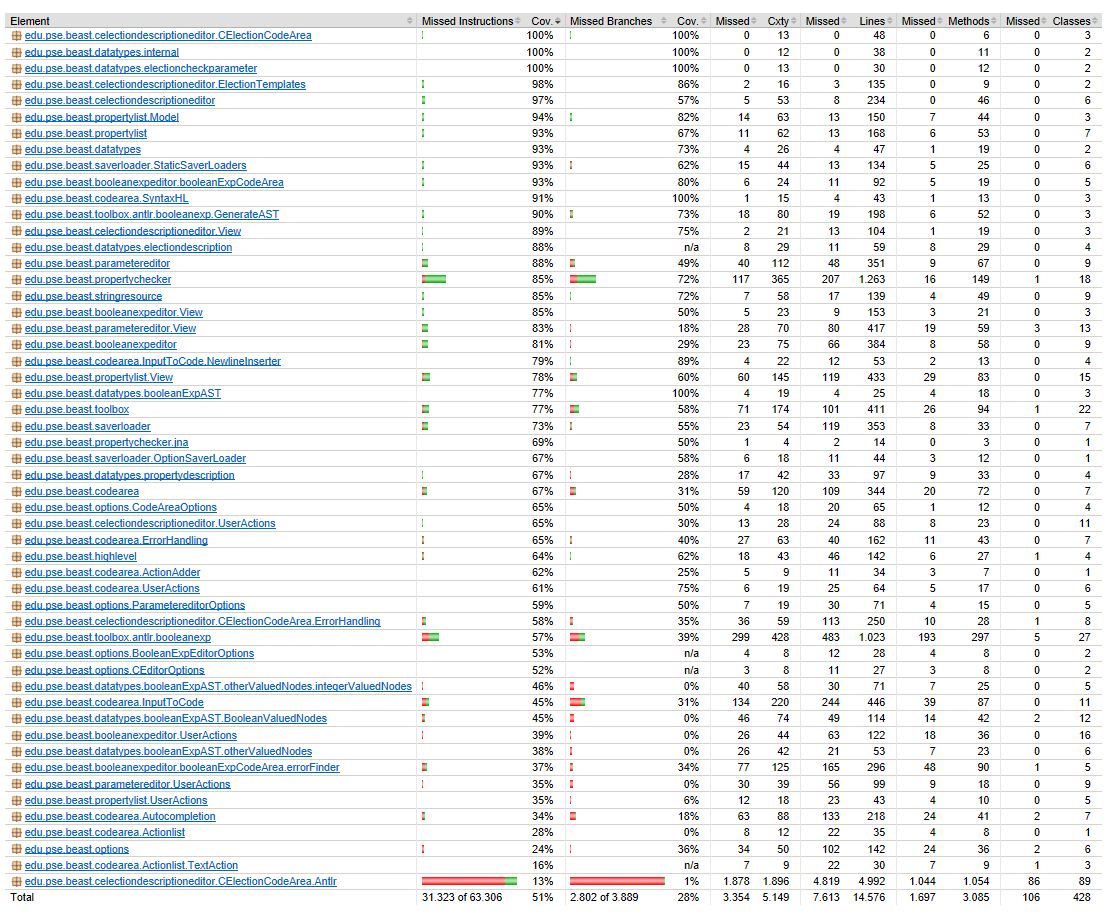
\includegraphics[width=1.0\textwidth,
  height=0.40\textwidth]{images/Coverage.png} \caption{Eine Übersicht über die
  in den einzelnen Paketen erreichte CodeCoverage (eine größere Version des
  Bildes befindet sich im Anhang)}
	\label{coverage}
\end{figure}



\section{Unit-Tests für AST- und Codegenerierung}
Da die theoretische Anzahl möglicher korrekter boolscher Ausdrücke abzählbar unendlich ist, ist es unmöglich jeden möglichen Ausdruck auf korrekte Übersetzung in AST und C-Code zu überprüfen. Daher wird stattdessen die AST- und Codegenerierung jedes Sprachkonstrukts einmal auf Korrektheit überprüft. 

Sprachkonstrukte sind im Pflichtenheft in "'1.1 Die Syntax zur Angabe der formalen Eigenschaften"' beschrieben. Zusätzlich werden einige gängige komplexere Ausdrücke überprüft (Beispiele in https://formal.iti.kit.edu/teaching/pse/201617/voting/kickOff.pdf, Folie 22). 

Zur Überprüfung der ASTs wurde Funktionalität zur Darstellung eines ASTs in textueller Form implementiert. Diese Repräsentation wird auf Korrektheit überprüft. Die Codegenerierung wird so getestet, dass ein gegebener boolscher Ausdruck übersetzt wird. Dadurch wird bei der Überprüfung der Codegenerierung erneut die Erstellung der ASTs überprüft. 

\chapter{Performance und Verbrauch:}
Über die Phase hinweg haben wir unser Programm stetig in einem Profiler betrachtet, um
schnell reagieren zu können, sollte eine Änderung in dieser Phase die
Lauffähigkeit unseres Programmes stärker als erwartet beeinflussen.

Das war jedoch nicht der Fall, sodass der Ressourcenverbrauch vor und nach der
Qualitätssicherungsphase relativ konstant geblieben ist.

Wie man in \ref{fig1} und \ref{fig2} erkennen kann, ist der Verlauf des
Speicherverbrauches so gut wie identisch mit ca. 30MB, bevor der "`garbage
collector"' es wieder auf ca. 10 MB herunterbringt. Anscheinend haben viele
unserer Objekte nur eine kurze Lebensdauer, woraus sich auch schließen ließe,
dass unser Programm im "`Leerlauf"' einen insignifikanten Speicherverbrauch hat,
der Computersysteme von heute vor keine große Aufgabe stellen sollte.

Vergleicht man nun \ref{fig3} mit \ref{fig4} sieht man, dass sich die
Unterschiede der Versionen, während eine Eigenschaft überprüft wird, schon
stärker unterscheiden. Während der Arbeitsspeicherverbrauch zwar noch relativ
ähnlich zwischen den beiden Versionen ist, sieht man, dass die Auslastung des
Prozessors schon deutliche Unterschiede aufweist. Diese Unterschiede sind jedoch vor allem darauf
zurückzuführen, dass nicht die exakt gleichen Wahlverfahren verglichen
wurden, weil sich im Laufe der Qualitätssicherungsphase etwas am System zum
Speichern der Wahlverfahren geändert hatte.

Der Grundfür den höheren Ressourcenverbrauch bei der Überprüfung ist, dass in dieser Phase zum einen der Code, welcher an CBMC gesendet
werden muss, für jede Eigenschaft einzeln erzeugt wird. Auch müssen mehrere Threads
konstant die Ausgabe von CBMC auffangen.
Ist die Überprüfung jedoch abgeschlossen normalisiert sich der
Ressourcenverbrauch wieder relativ schnell.

\newpage
\begin{figure}[ht]
	\centering
  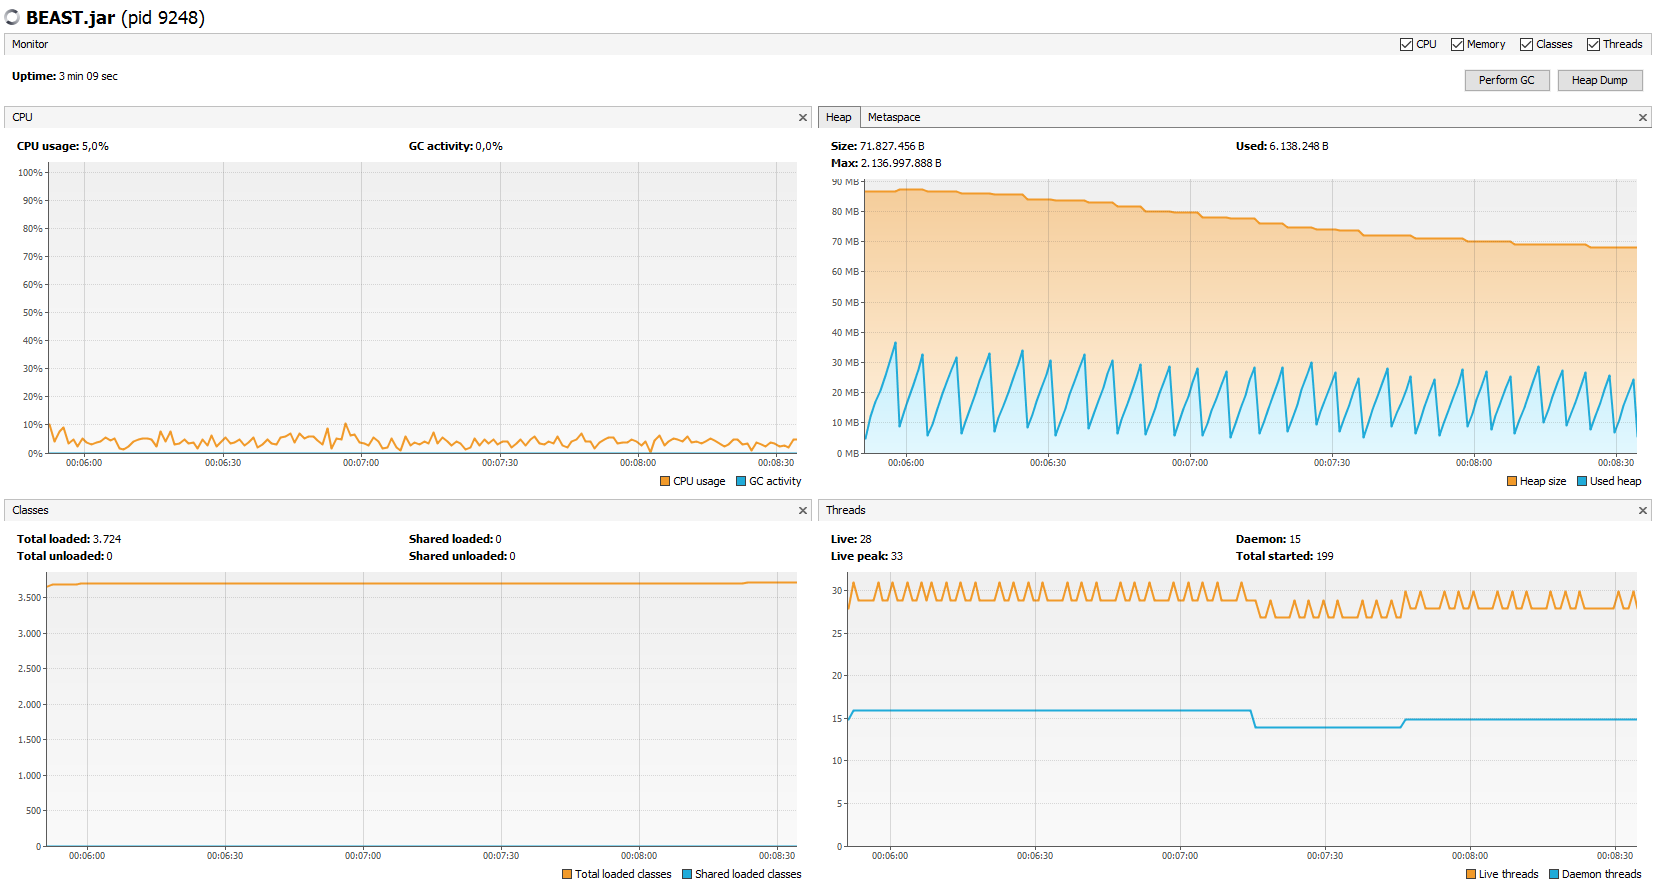
\includegraphics[width=1.0\textwidth,
  height=0.40\textwidth]{images/OLD_NO.png} \caption{Dies ist der
  Ressourcenverbrauch des Programmes, während es auf eine Eingabe vom Nutzer wartet und momentan keine Verifikation durchführt}
	\label{fig1}
\end{figure}

\vspace{4cm}

\begin{figure}[ht]
	\centering
  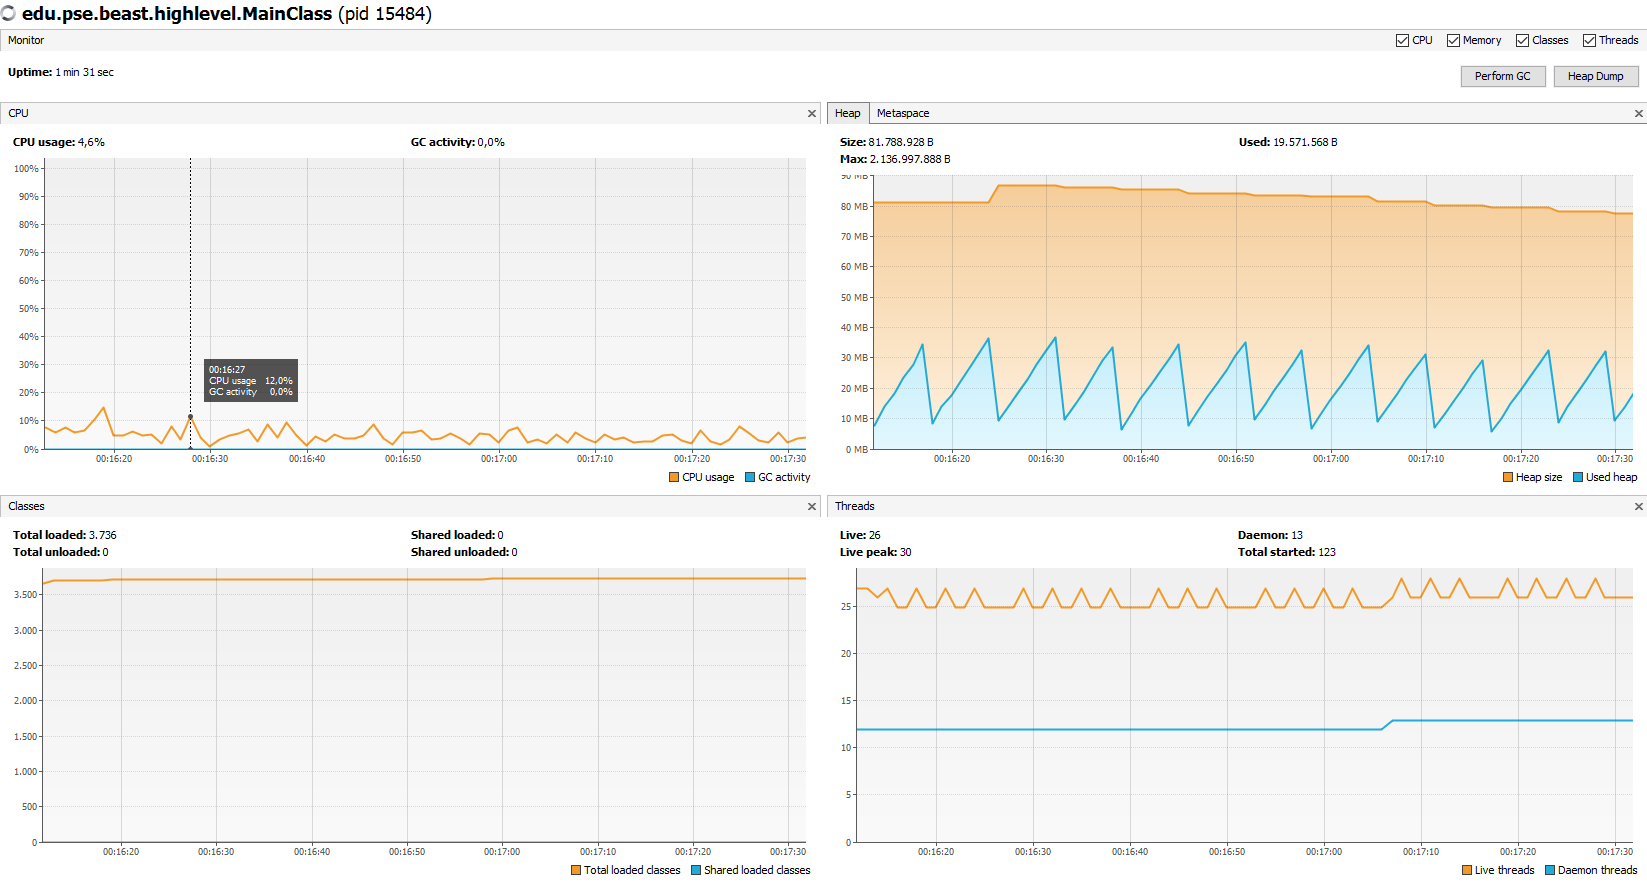
\includegraphics[width=1.0\textwidth,
  height=0.40\textwidth]{images/NEW_NO.png} \caption{Der Ressourcenverbrauch der
  momentanen Version des Programmes, während keine Überprüfung durchgeführt wird}
	\label{fig2}
\end{figure}


\newpage

\begin{figure}[ht]
	\centering
  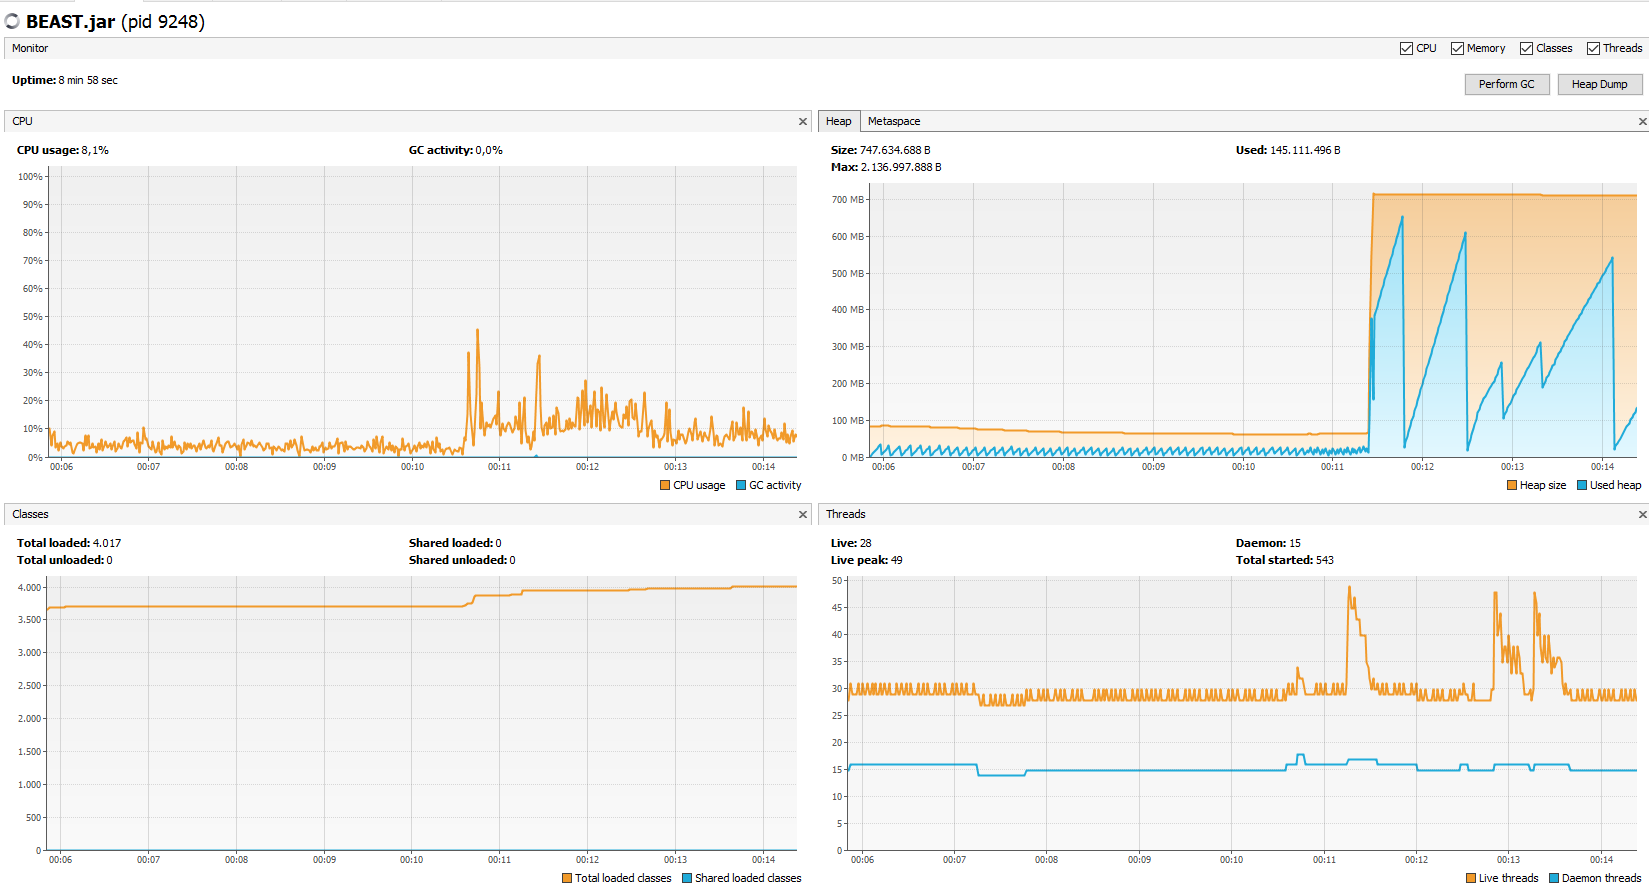
\includegraphics[width=1.0\textwidth,
  height=0.4\textwidth]{images/OLD_YES.png} \caption{Der Ressourcenverbrauch
 der originalen Version von BEAST, während Eigenschaften überprüft werden}
	\label{fig3}
\end{figure}

\vspace{4cm}

\begin{figure}[ht]
	\centering
  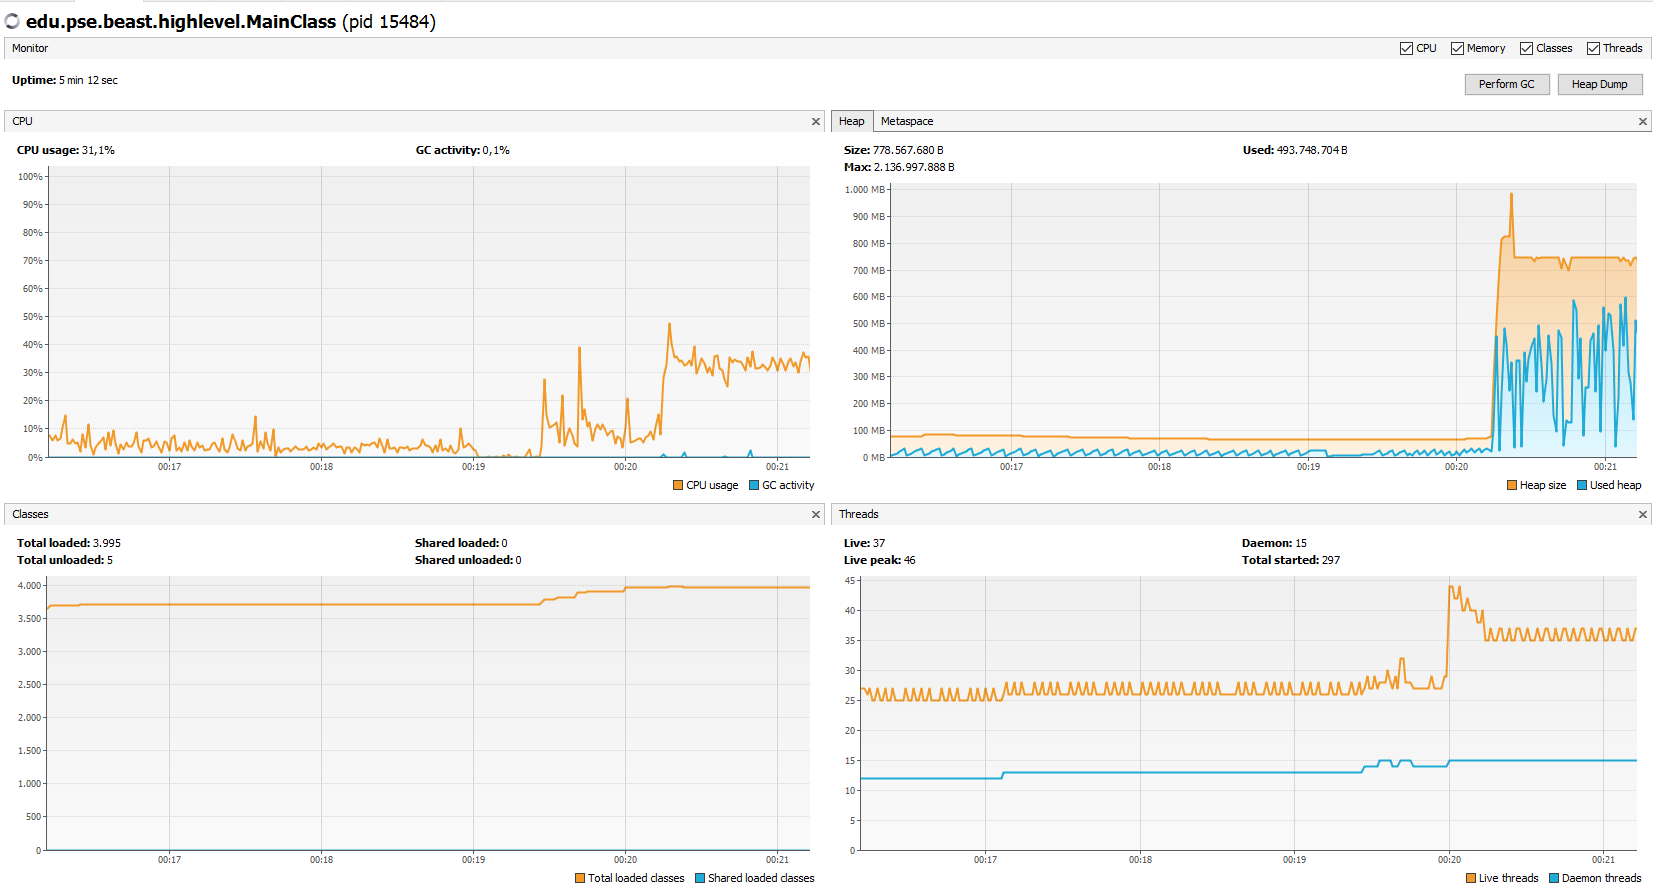
\includegraphics[width=1.0\textwidth,
  height=0.40\textwidth]{images/NEW_YES.png} \caption{Der Ressourcenverbrauch der
  momentanen Version des Programmes, während Eigenschaften überprüft werden}
	\label{fig4}
\end{figure}

\newpage
Betrachtet man die Verteilung der Prozessorzeit der neusten BEAST-Version während einer
Analyse (siehe \ref{fig5}) fällt auf, dass die Methoden, welche die meiste
Zeit in Anspruch nehmen, die sind, die dafür sorgen, dass das Programm
so angenehm wie möglich läuft. Würde man zum Beispiel die konstante
Überprüfung auf Fehler weniger häufig ausführen, müsste der Nutzer länger auf eine
Rückmeldung warten, was er noch ändern müsste. 

Ähnlich verhält es sich zu den
"`ThreadedBufferedReader"'-Instanzen, die auch noch einen großen Anteil an der
Prozessorzeit haben. Dies liegt daran, dass sie die gesamte Kommunikation zu
außerhalb laufenden Prozessen übernehmen, und deshalb die gesamte Zeit ohne
Unterbrechung laufen müssen, solange der Prozess, den sie überwachen, auch noch
läuft.

\begin{figure}[ht]
	\centering
  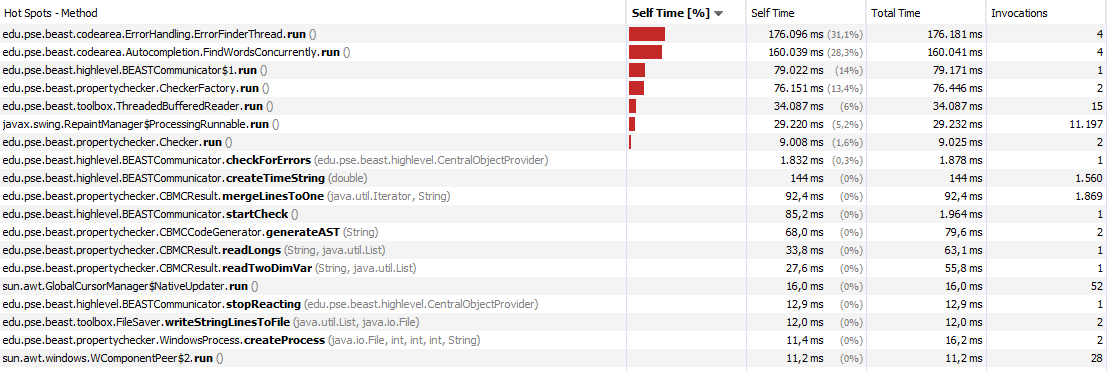
\includegraphics[width=1.0\textwidth,
  height=0.40\textwidth]{images/BEAST_PROCESSORTIME.png} \caption{Der
  prozentuale Anteil einzelner Methoden an der gesamten genutzten Prozessorzeit}
	\label{fig5}
\end{figure}

\chapter{Fehlerbehebungen}
Im Laufe der Phase haben wir einige Fehler gefunden, welche die Benutzung von
BEAST stark beeinträchtigt haben. Eine komplette Liste aller "`Issues"' kann auf
der BEAST
GitHub-Seite\footnote{https://github.com/NikolaiLMS/PSE-Wahlverfahren-Implementierung/issues}
angeschaut werden. Trotzdem werden wir hier einen kleinen Überblick über ein
paar der gefundenen Fehler und deren Behebung geben:

\paragraph{Issue 16}- \newline
Beschreibung: Es war möglich, Zeilen zu verändern, welche als nicht editierbar angezeigt und festgelegt wurden. Dies geschah, wenn man unterhalb einer solchen Zeile etwas schrieb. Durch Entfernen des Zeilentrennungszeichens wurde dieses Zeichen dann in die nicht editierbare Zeile angehoben.
\newline
Lösung: In die \verb!removeToTheLeft! Methode in \verb!UserInserToCode! wurde ein zusätzlicher Check eingefügt. Es überprüft nun, ob die Zeile über der, in welcher etwas gelöscht wird, nicht editierbar ist. Falls ja, und das zu löschende Zeichen ist ein Zeichentrennungszeichen, wird nur gelöscht, falls die Zeile leer ist, auf welcher sich der Cursor befindet.

\paragraph{Issue 17}- \newline
Beschreibung: Öffnet man eine falsch formatierte Datei in BEAST führte dies zu
einer NullpointerException
\newline
Lösung: Gelöst durch zwingende Namensgebung der form
"`list_of_candidates_per_voter"' 

\paragraph{Issue 27}- \\
Beschreibung: Obwohl als Voraussetzung angegeben war, dass beide vote-Arrays gleich sein sollten (\verb!VOTES1==VOTES2!) wurden in beiden Wahlvorgängen verschiedene Stimmen abgegeben.\\
Lösung: Der Bug stammte daher, dass der generierte Code die abgegebenen Stimmen nur bis zur Anzahl der Wähler verglich. Bei Wahlverfahren, bei welchen jeder Wähler eine Liste mit Länge der Anzahl von Kandidaten abgibt, wurden daher nur die ersten Stimmen verglichen. Dies führte zu dem Bug, sobald es mehr Kandidaten als Wähler gab.

\paragraph{Issue 28}- \\
Beschreibung: Bei einem Wahlverfahren, welches Preference-Voting als Input verwendet, dauerte es enorm lange eine Eigenschaft zu testen, wenn es mehr Kandidaten als Wähler gab. Bei 6 Wählern und Kandidaten dauerte eine Überprüfung wenige Sekunden. Bei 5 Wählern und 6 Kandidaten war die Überprüfung nach 2 Minuten noch nicht fertig.\\
Lösung: Die Ursache war, dass bei Preference-voting als zusätzliche Voraussetzung alle von einem Wähler abgegebenen Stimmen verschieden sein müssen. Dies liegt daran, dass diese Platzierungen von Wählern repräsentieren. Der Code, welcher produziert wurde, um diese Eigenschaft sicherzustellen, war fehlerhaft.

\paragraph{Issue 42}- \\
Beschreibung: Bei der Codeerzeugung für Vergleiche wurden linke und rechte Seite des Vergleichs vertauscht.\\
Lösung: An der Stelle, an welcher der String für den Vergleich generiert wird, wurde "`lhs"' und "`rhs"' vertauscht. 
 


\chapter{Verbesserungen in der Phase}
Neben Fehlerbehebungen haben wir BEAST in dieser Phase auch in einigen Punkten
verbessert:

\begin{itemize}
  \item Im Eigenschafteneditor gibt es nun einen Knopf, welcher eine Erklärung
  über die BooleanExpressionLanguage gibt, mit der der Nutzer seine Befehle
  schreiben kann.
  \item Der Nutzer kann nun Wähler, Kandidaten und Sitze via ihrer Position in den entsprechenden Arrays angeben. Dazu wurden die Sprachkonstrukte \verb!VOTER_AT_POS!, \verb!CAND_AT_POS! und \verb!SEAT_AT_POS! implementiert.
  \item Der Nutzer kann nun beliebige mathematische Terme angeben, welche *, /, + und - unterstützen. Diese binären mathematischen Operationen können auf sämtliche Ausdrücke angewendet werden, welche einen ganzzahligen Wert liefern.
  \item Gibt der Nutzer nun Dateien, welche in das C-Programm eingebunden werden
  sollen, an, wird automatisch überprüft, ob diese einem standart C-Include
  entsprechen, oder aber in dem speziellen Ordner \backslash core \backslash
  user_includes \backslash liegen. Sie werden dann auch automatisch an cbmc
  weitergegeben, sodass der nutzer keine weiteren Arbeiten machen muss, wenn er
  eine eigene Datei einbinden will.
\end{itemize}

\chapter{Anhang}

\section{Testprotokolle} 
\begin{table}[]
\caption{Testfall 8.1 (Testfälle für die Datenverwaltung)}
\centering
	\begin{tabular}{| p{0.10\linewidth} | p{0.15\linewidth} | p{0.27\linewidth} |
	p{0.15\linewidth} | p{0.09\linewidth} | p{0.09\linewidth} |}
	\hline
	\textbf{Sub-Testfall} &
	\textbf{Abgedeckte Funktionalitäten} &
	\textbf{Beschreibung} &
	\textbf{Ergebnis} & \textbf{Lukas}
	(Windows 10) Version 1.4.22 &
	\textbf{Justin} Lubuntu 16.1 Version 1.4.19
\\
\hline
/T010/ (C-Editor) &
/FS1030/ /FS1100/ /FS1110/ & 
Man gibt ein Wahlverfahren ein. Man wählt in der Toolbar den Button "`Neu"' aus. In einen Dialog gibt man das gewünschte Wahlverfahren und die Anzahl der Sitze ein. In ein Textfeld wird der Name eingegeben. Man drückt auf den Button "`Erstellen"'.
 &
Ein neuer vorgefertigter C-Code erscheint im C-Editor. Ausgegraut sind die Argumente des Wahlverfahrens. &
\Checkmark & \Checkmark
\\
\hline 
/T010/ (Eigenschafteneditor) &
/FM2100/ /FS2150/ &
Man gibt formale Eigenschaften ein. Man wählt in der Toolbar den Button "`Neu"' aus. 
 &
Die Felder für "`Symbolische Variablen"', "`Vorbedingungen"' und "`Nachbedingungen"' leeren sich. In der Titelleiste erscheint der Name "`Eigenschaft 0"'. &
\centering \Checkmark & \Checkmark
\\
\hline 
/T010/ (Eigenschaftenliste) &
/FM3020/ &
Man fügt Eigenschaften zur Liste hinzu. Man wählt in der Toolbar den Button "`Neu"' aus. Die Nachfrage, ob man speichern will, wird verneint.
 &
Die Liste der Eigenschaften leert sich. &
\Checkmark & \Checkmark
\\
\hline 
/T010/ (Parametereditor) &
/FM4050/ &
Man ändert die Parameter. Man wählt in der Toolbar den Button "`Neu"' aus.
 &
Es existiert kein Button für das Neu erstellen. &
X & X
\\
\hline



\end{tabular}
\end{table}
\begin{table}[]
\caption{Testfall 8.1 (Testfälle für die Datenverwaltung)}
\centering
	\begin{tabular}{| p{0.15\linewidth} | p{0.15\linewidth} | p{0.20\linewidth} |
	p{0.15\linewidth} | p{0.1\linewidth} | p{0.1\linewidth} |}
	\hline
	\textbf{Sub-Testfall} &
	\textbf{Abgedeckte Funktionalitäten} &
	\textbf{Beschreibung} &
	\textbf{Ergebnis} & \textbf{Lukas}
	(Windows 10) Version ??? &
	\textbf{Justin} Lubuntu 16.1 Version 1.4.19) 
\\
\hline
/T020/ /T030/ (C-Editor) &
/FM1030/ /FS1100/ /FS1040/ /FS1060/ &
Man gibt ein Wahlverfahren ein. Man wählt in der Toolbar den Button "`Speichern"' aus. In einen Dialog gibt man den gewünschten Speicherort ein. Man drückt auf den Button "`Speichern"'. Man wählt in der Toolbar den Button "`Öffnen"' aus. In einem Dialog wählt man das gespeicherte Wahlverfahren aus.
 &
Das Wahlverfahren wurde gespeichert. Das Laden des Wahlverfahrens schlug fehl. Das Format wurde nicht erkannt. &
\centering . & X
\\
\hline 
/T020/ /T030/ (Eigenschafteneditor) &
/FM2100/ /FS2110/ &
Man gibt formale Eigenschaften ein. Man wählt in der Toolbar den Button "`Speichern"' aus. In einen Dialog gibt man den gewünschten Speicherort ein. Man drückt auf den Button "`Speichern"'. Man wählt in der Toolbar den Button "`Öffnen"' aus. In einem Dialog wählt man die gespeicherten formalen Eigenschaften aus.
 &
Die Eigenschaft wurde gespeichert. Das Laden schlägt fehl. Das Format wurde nicht erkannt. &
\centering . & X
\\
\hline 


\end{tabular}
\end{table}
\begin{table}[]
\caption{Testfall 8.1 (Testfälle für die Datenverwaltung)}
\centering
	\begin{tabular}{| p{0.15\linewidth} | p{0.15\linewidth} | p{0.20\linewidth} |
	p{0.15\linewidth} | p{0.1\linewidth} | p{0.1\linewidth} |}
	\hline
	\textbf{Sub-Testfall} &
	\textbf{Abgedeckte Funktionalitäten} &
	\textbf{Beschreibung} &
	\textbf{Ergebnis} & \textbf{Lukas}
	(Windows 10) Version ??? &
	\textbf{Justin} Lubuntu 16.1 Version 1.4.19) 
\\
\hline 
/T020/ /T030/ (Eigenschaftenliste) &
/FM3060/ /FM3070/ &
Man fügt Eigenschaften zur Liste hinzu. Man wählt in der Toolbar den Button "`Speichern"' aus. In einen Dialog gibt man den gewünschten Speicherort ein. Man drückt auf den Button "`Speichern"'. Man wählt in der Toolbar den Button "`Öffnen"' aus. In einem Dialog wählt man die gespeicherte Eigenschaftenliste aus.
 &
Die Liste der Eigenschaften wurde gespeichert. Die Liste wird wieder geladen. &
\centering . & \Checkmark
\\
\hline 
/T020/ /T030/ (Parametereditor) &
/FM4050/ /FM4060/ &
Man ändert die Parameter. Man wählt in der Toolbar den Button "`Speichern"' aus. In einen Dialog gibt man den gewünschten Speicherort ein. Man drückt auf den Button "`Speichern"'. Man wählt in der Toolbar den Button "`Öffnen"' aus. In einem Dialog wählt man die gespeicherte Eigenschaftenliste aus.
 &
Das Projekt wird gespeichert. Das Projekt kann wieder geladen werden. &
\centering . & \Checkmark
\\ \hline 

\end{tabular}
\end{table}
\begin{table}[]
\caption{Testfall 8.2 (Testfall für Rückgängig machen und Wiederherstellen)}
\centering
	\begin{tabular}{| p{0.15\linewidth} | p{0.15\linewidth} | p{0.20\linewidth} |
	p{0.15\linewidth} | p{0.1\linewidth} | p{0.1\linewidth} |}
	\hline
	\textbf{Sub-Testfall} &
	\textbf{Abgedeckte Funktionalitäten} &
	\textbf{Beschreibung} &
	\textbf{Ergebnis} & \textbf{Lukas}
	(Windows 10) Version 1.4.13 &
	\textbf{Niels} (Linux Mint Cinnamon 3.0.7) Version 1.4.22 
\\
\hline
/T100/ &
/FS1100/ /FS2150/ /F0010/ /F0050/ &
Man startet das Programm ganz normal. Nun gibt man in
jedes Feld, das die "`Rückgängig machen"' Funktionalität unterstützt, einen
kleinen Text ein, und drückt dann, während der Fokus auf dem zu testendem Feld
liegt "`Strg + z"'. &
Der zuletzt eingegebene Buchstabe
oder Textblock (im Falle des Einfügens mit "`Strg + v"') wird gelöscht. &
\Checkmark & \Checkmark 
\\
\hline /T110/& /FS1100/ /FS2150/ /F0010/ /F0050 &
Man startet das Programm ganz normal. Nun gibt man in
jedes Feld, das die "`Rückgängig machen"' Funktionalität unterstützt, einen
kleinen Text ein, und drückt dann, während der Fokus auf dem zu testendem Feld
liegt "`Strg + z"'. Nun drückt man "`Strg + r". &
Der vorher durch das rückgängig machen verschwundene Buchstabe oder Textblock
erscheint wieder. &
\Checkmark 
& \Checkmark  
\\ \hline

\end{tabular}
\end{table}


\begin{table}[]
\caption{Testfall 8.3 (Testfall für Kopieren, Einfügen und Ausschneiden in den Editoren)}
\centering
	\begin{tabular}{| p{0.09\linewidth} | p{0.14\linewidth} | p{0.27\linewidth} |
	p{0.15\linewidth} | p{0.1\linewidth} | p{0.1\linewidth} |}
	\hline
	\textbf{Sub-Testfall} &
	\textbf{Abgedeckte Funktionalitäten} &
	\textbf{Beschreibung} &
	\textbf{Ergebnis} & \textbf{Niels}
	(Windows 10) Version 1.4.22 &
	\textbf{Niels} (Linux Mint Cinnamon 3.0.7) Version 1.4.22
\\
\hline
/T200/ &
/F0010/ /FS1100/ /FS2150/ &
Man startet das Programm ganz normal. Nun öffnet man den den jeweiligen Editor (C-Editor und Eigenschafteneditor) und gibt einen kleinen Text ein.
Man markiert den kleinen Text und drückt dann, während der Fokus auf dem Editor liegt, "`Strg + x"' oder betätigt den Button für Ausschneiden. 
&
Der markierte Text wird gelöscht und in den Zwischenspeicher gespeichert. &
\Checkmark & \Checkmark
\\
\hline
/T200/ &
/F0010/ /FS1100/ /FS2150/ &
Man startet das Programm ganz normal. Nun öffnet man den den jeweiligen Editor (C-Editor und Eigenschafteneditor) und gibt einen kleinen Text ein.
Man markiert den kleinen Text und drückt dann, während der Fokus auf dem Editor liegt, "`Strg + c"' oder betätigt den Button für Kopieren
&
Der markierte Text wird in den Zwischenspeicher gespeichert. &
\Checkmark & \Checkmark
\\
\hline
/T200/ &
/F0010/ /FS1100/ /FS2150/ &
Man startet das Programm ganz normal. Nun öffnet man den den jeweiligen Editor (C-Editor und Eigenschafteneditor)
Man drückt "`Strg + v"' oder betätigt den Button für Einfügen.
&
Falls ein Text im Zwischenspeicher gespeichert ist, wird er im Editor eingefügt. &
\Checkmark & \Checkmark
\\
\hline

\end{tabular}
\end{table}
\begin{table}[]
\caption{Testfall 7 (Nichtfunktionale Anforderungen)}
\centering
	\begin{tabular}{| p{0.09\linewidth} | p{0.14\linewidth} | p{0.21\linewidth} |
	p{0.21\linewidth} | p{0.1\linewidth} | p{0.1\linewidth} |}
	\hline
	\textbf{Sub-Testfall} &
	\textbf{Abgedeckte Funktionalitäten} &
	\textbf{Beschreibung} &
	\textbf{Ergebnis} & \textbf{Lukas}
	(Windows 10) Version 1.4.22 &
	\textbf{Niels} (Linux Mint Cinnamon 3.0.7) Version 1.4.22
\\
\hline
 &
/NF10/ &
Man startet das Programm ganz normal. Nun öffnet man den C-Editor und gibt in
die Mitte der Voting Methode "`for"' ein. Nun drückt man "`strg"' +
"`leer"' & In weniger als 0.5 Sekunden öffnet sich ein Fenster, welches die
Code-Completion anzeigt & \Checkmark & \Checkmark
\\
\hline
 &
/NF30/ &
Man startet das Programm ganz normal und öffnet den C-Editor. Hier gibt man nun
einen Code ein, der über 10000 Zeilen lang ist. Im ParameterEditor wählt man
alle Variablen kleiner als 10 und stellt den TimeOut aus. Im Eigenschafteneditor
öffnet man "`FalseProperty.props"'. Nun startet man die Überprüfung & Nach
kurzer Zeit beendet sich die Überprüfung, und man kan das Ergebnis im
Eigenschafteneditor ablesen & \Checkmark &
\Checkmark
\\
\hline
 &
/NF20/ /NF40/ /NF50/ /NF60/ &
Man startet das Programm ganz normal und öffnet den C-Editor. Hier gibt man nur
einen sehr einfachen Code ein. Im Eigenschafteneditor erstellt man eine neue
Eigenschaft, welche 10 Vor- und Nachbedingungen enthält. Im Parametereditor
stellt man alle Werte auf 10000, und den TimeOut auf 15 Minuten & CBMC startet
mit der Überprüfung der Eigenschaft. Nach 15 Minuten hört es mit der Überprüfung
auf. & \Checkmark &
\Checkmark
\\
\hline
\end{tabular}
\end{table}

\begin{table}[]
\caption{Testfall 8.3 (Bearbeiten des Codes in den Editoren)}
\centering
	\begin{tabular}{| p{0.09\linewidth} | p{0.14\linewidth} | p{0.21\linewidth} |
	p{0.21\linewidth} | p{0.1\linewidth} | p{0.1\linewidth} |}
	\hline
	\textbf{Sub-Testfall} &
	\textbf{Abgedeckte Funktionalitäten} &
	\textbf{Beschreibung} &
	\textbf{Ergebnis} & \textbf{Niels}
	(Windows 10) Version 1.4.22 &
	\textbf{Niels} (Linux Mint Cinnamon 3.0.7) Version 1.4.22
\\
\hline
/T210/ &
/FS1130/ /FK2140/ &
Man startet das Programm ganz normal. Nun öffnet man den den jeweiligen Editor (CEditor und Eigenschafteneditor) und gibt ein Wort innerhalb des Editors teilweise ein, dass der richtigen Syntax entspricht. Nun betätigt man "`Strg + Leertaste"'
&
Es öffnet sich ein Fenster für die Autocompletion, aus der man die gewünschte Eingabe wählen kann, welche nach Auswahl hinzugefügt wird.   &
\Checkmark & \Checkmark
\\

\hline
/T210/ &
/FS1120/ /FS1130/ &
Man startet das Programm ganz normal. Man öffnet den C-Editor. Man gibt C-Code ein. 
&
Klammern und Anführungszeichen werden automatisch geschlossen.
Code in Schleifen und if-Statements wird automatisch eingerückt. &
\Checkmark & \Checkmark
\\
\hline

\end{tabular}
\end{table}

\begin{table}[]
\caption{Testfälle 8.4 (Testfälle für den C-Editor)}
\centering
	\begin{tabular}{| p{0.15\linewidth} | p{0.15\linewidth} | p{0.20\linewidth} |
	p{0.15\linewidth} | p{0.1\linewidth} | p{0.1\linewidth} |}
	\hline
	\textbf{Sub-Testfall} &
	\textbf{Abgedeckte Funktionalitäten} &
	\textbf{Beschreibung} &
	\textbf{Ergebnis} & \textbf{Holger} Windows 7  &
	\textbf{Holger} Ubuntu (16.04 LTS))
\\
\hline
/T310/ &
/FS1110/&
Man startet das Programm und öffnet den C-Editor. Dort wählt man eine der Möglichkeiten eine neue Wahlbeschreibung zu entwerfen
&
& 
&
\\
\hline
&
/FS1100/&
Per Shortcut: Strg + n
& Der Dialog zum Erstellen einer neuen Wahlverfahrensbeschreibung wird angezeigt
& \Checkmark
&\Checkmark
\\
\hline
&
&
Per Menü: Datei, dann Neu
& Der Dialog zum Erstellen einer neuen Wahlverfahrensbeschreibung wird angezeigt
& \Checkmark
&\Checkmark
\\
\hline
&
&
Per Toolbar: Erster Button der Toolbar
& Der Dialog zum Erstellen einer neuen Wahlverfahrensbeschreibung wird angezeigt
& \Checkmark
&\Checkmark
\\
\hline
\end{tabular}
\end{table}

\begin{table}[]
\caption{Testfälle 8.4 (Testfälle für den C-Editor)}
\centering
	\begin{tabular}{| p{0.15\linewidth} | p{0.15\linewidth} | p{0.20\linewidth} |
	p{0.15\linewidth} | p{0.1\linewidth} | p{0.1\linewidth} |}
	\hline
	\textbf{Sub-Testfall} &
	\textbf{Abgedeckte Funktionalitäten} &
	\textbf{Beschreibung} &
	\textbf{Ergebnis} & \textbf{Holger} Windows 7 &
	\textbf{Holger} Ubuntu (16.04 LTS))
\\
\hline
& /FS1110/
& Auswahl eines Input- und Resulttypen sowie eines Namens. Klicken des "Erstellen"-Buttons
& Der Funktionskörper wird entsprechend aktualisiert 
& 
&
\\
\hline
&
& Single-choice 
& Input: unsigned int votes[V]
& \Checkmark
& \Checkmark
\\
\hline
&
& Preference 
& Input: unsigned int votes[V][C]
& \Checkmark
& \Checkmark
\\
\hline
&
& Approval 
& Input: unsigned int votes[V][C]
& \Checkmark
& \Checkmark
\\
\hline
&
& Weighted Approval 
& Input: unsigned int votes[V][C]
& \Checkmark
& \Checkmark
\\
\hline
&
& Candidate or not determined
& Result: unsigned int 
& \Checkmark
& \Checkmark
\\
\hline
&
& Seats per party
& Result: unsigned int *
& \Checkmark
& \Checkmark
\\
\hline
\end{tabular}
\end{table}

\begin{table}[]
\caption{Testfälle 8.4 (Testfälle für den C-Editor)}
\centering
	\begin{tabular}{| p{0.15\linewidth} | p{0.15\linewidth} | p{0.20\linewidth} |
	p{0.15\linewidth} | p{0.1\linewidth} | p{0.1\linewidth} |}
	\hline
	\textbf{Sub-Testfall} &
	\textbf{Abgedeckte Funktionalitäten} &
	\textbf{Beschreibung} &
	\textbf{Ergebnis} & \textbf{Holger} Windows 7 &
	\textbf{Holger} Ubuntu (16.04 LTS))
\\
\hline
/T320/ &
/FM1050/&
Man startet das Programm und öffnet den C-Editor. Dort gibt man ein Programm ein welches mehrere Fehler enthält. Danach wählt man im Menü Code "statische Analyse" aus.
Fehler: Fehlendes return, Zugriff auf nicht deklarierte Variable, Verwendung nicht deklarierter Funktion, Funktionsaufruf mit falschen Parametern, fehlendes Semikolon, Fehlende schließende geschweifte Klammer nach for-Schleife
& Es werden alle Fehler im Code angezeigt
& \Checkmark
& \Checkmark
\\
\hline
\end{tabular}
\end{table}

\begin{table}[]
\caption{Testfälle 8.4 (Testfälle für den C-Editor)}
\centering
	\begin{tabular}{| p{0.15\linewidth} | p{0.15\linewidth} | p{0.20\linewidth} |
	p{0.15\linewidth} | p{0.1\linewidth} | p{0.1\linewidth} |}
	\hline
	\textbf{Sub-Testfall} &
	\textbf{Abgedeckte Funktionalitäten} &
	\textbf{Beschreibung} &
	\textbf{Ergebnis} & \textbf{Holger} Windows 7 &
	\textbf{Holger} Ubuntu (16.04 LTS))
\\
\hline
&
/FM1030/, /FM1040/&
Man startet das Programm und öffnet den C-Editor. Dort speichert man die geöffnete Wahlverfahrensbeschreibung an. einem beliebigen Ort. Danach klickt man auf Öffnen, navigiert an den Ort an dem die Datei gerade gespeichert wurde, und öffnet sie 
& Die gespeicherte Datei wird angezeigt
& \Checkmark
& \Checkmark
\\
\hline
\end{tabular}
\end{table}

\begin{table}[]
\caption{Testfälle 8.4 (Testfälle für den C-Editor)}
\centering
	\begin{tabular}{| p{0.15\linewidth} | p{0.15\linewidth} | p{0.20\linewidth} |
	p{0.15\linewidth} | p{0.1\linewidth} | p{0.1\linewidth} |}
	\hline
	\textbf{Sub-Testfall} &
	\textbf{Abgedeckte Funktionalitäten} &
	\textbf{Beschreibung} &
	\textbf{Ergebnis} & \textbf{Holger} Windows 7 &
	\textbf{Holger} Ubuntu (16.04 LTS))
\\
\hline
&
/FK1130/&
Man startet das Programm und öffnet den C-Editor. Dort geht man in den Körper der voting-Funktion und beginnt return zu tippen. Nach den ersten zwei Buchstaben betätigt man den Shortcut Strg - Leer. In dem erschienenen Menü wählt man return aus und drückt Enter.
& Das Wort return wird in den Funktionskörper geschrieben
& \Checkmark
& \Checkmark
\\
\hline
&
/FK1130/&
Man gibt in den Funktionskörper der voting-Funktion den text int asdasdasd ein und wartet 10 Sekunden. Danach geht man auf eine neue Zeile und tippt a. Dann betätigt man den Shortcut Strg-Leer
& In dem erschienenen Menü wird nun asdasdasd als Option angezeigt
& \Checkmark
& \Checkmark
\\
\hline
\end{tabular}
\end{table}

\begin{table}[]
\caption{Testfälle 8.4 (Testfälle für den C-Editor)}
\centering
	\begin{tabular}{| p{0.15\linewidth} | p{0.15\linewidth} | p{0.20\linewidth} |
	p{0.15\linewidth} | p{0.1\linewidth} | p{0.1\linewidth} |}
	\hline
	\textbf{Sub-Testfall} &
	\textbf{Abgedeckte Funktionalitäten} &
	\textbf{Beschreibung} &
	\textbf{Ergebnis} & \textbf{Holger} Windows 7 &
	\textbf{Holger} Ubuntu (16.04 LTS))
\\
\hline
&
/FK1140/&
Man startet das Programm und öffnet den C-Editor. Dort geht man auf den Menüpunkt Editor -> Eigenschaften. In dem erschienenen Dialog wählt man einen anderen Font und Schriftgröße aus
& Der verwendete Font und Schriftgröße werden zu der gewählten aktualisiert. Diese Änderung bleibt auch nach Neustart des Programmes
& \Checkmark
& \Checkmark
\\
\hline
\end{tabular}
\end{table}
\begin{table}[]
\caption{Testfall 8.5 (Testfall für das Erstellen einer Eigenschaft im Eigenschafteneditor)}
\centering
	\begin{tabular}{| p{0.15\linewidth} | p{0.15\linewidth} | p{0.20\linewidth} |
	p{0.15\linewidth} | p{0.1\linewidth} | p{0.1\linewidth} |}
	\hline
	\textbf{Sub-Testfall} &
	\textbf{Abgedeckte Funktionalitäten} &
	\textbf{Beschreibung} &
	\textbf{Ergebnis} & \textbf{Lukas}
	(Windows 10) Version 1.4.22 &
	\textbf{Nikolai} Arch Linux (4.10.3-1-ARCH))
\\
\hline
/T410/ &
/FM2040/ /FM2050/ /FM2070/ /FM2071/ /FM2072/ /FM2073/ /FM2080/ /FM2100/ /FM2120/&
Man startet das Programm ganz normal. Nun gibt man im Eigenschafteneditor in den Vorbedingungen 'VOTES1 == VOTES2;', und in den Nachbedingungen 'ELECT1 != ELECT2;' ein. Durch auswählen von "Statische Fehlersuche" testet man die Eigenschaft auf Korrektheit und kann diese anschließend mit dem entsprechenden Menüpunkt oder Toolbar-Button speichern. &
Es wird 'Fehler: 0' im Fehlerfenster angezeigt und die Eigenschaft hat sich ohne Fehlermeldung speichern lassen. &
\Checkmark & \Checkmark
\\
\hline

\end{tabular}
\end{table}
\begin{table}[]
\caption{Testfall 8.6 (Testfälle für die Eigenschaftenliste)}
\centering
	\begin{tabular}{| p{0.10\linewidth} | p{0.15\linewidth} | p{0.27\linewidth} |
	p{0.15\linewidth} | p{0.09\linewidth} | p{0.09\linewidth} |}
	\hline
	\textbf{Sub-Testfall} &
	\textbf{Abgedeckte Funktionalitäten} &
	\textbf{Beschreibung} &
	\textbf{Ergebnis} & \textbf{Lukas}
	(Windows 10) Version 1.4.22 &
	\textbf{Justin} Lubuntu 16.1 Version 1.4.19) 
\\
\hline
/T510/ &
/FM0010/ /FM0020/ /FM0030/ /FM0031/ &
Man gibt ein einfaches Wahlverfahren ein, das eine gewählte Person zurückgibt. Man erstellt eine erste Eigenschaft, die erfüllt ist, und eine zweite Eigenschaft, die nicht erfüllt ist. Man wählt im Parametereditor den Start der Analyse in der Toolbar aus.
 &
Die erste Eigenschaft erscheint grün. Die zweite Eigenschaft erscheint rot. Beim Klick auf das Augensymbol der zweiten Eigenschaft öffnet sich ein Fenster mit einem Gegenbeispiel. &
\Checkmark & \Checkmark
\\
\hline 
/T520/ &
/FM3010/ /FM3050/ &
Man fügt der Eigenschaftenliste eine Eigenschaft hinzu, indem man auf den Button mit dem Pluszeichen und der Beschriftung "`Neu"' drückt. Die Checkbox mit der Beschriftung "`Analyse"' klickt man an. Man wählt im Parametereditor den Start der Analyse in der Toolbar aus.
 &
Die Eigenschaft erscheint grün. Die Eigenschaft wurde von CBMC überprüft. &
\Checkmark & \Checkmark
\\
\hline 
/T530/ &
/FM3010/ FM3020/ &
Man drückt auf den Button mit dem Pluszeichen und der Beschriftung "`Neu"'. 
 &
Eine neue Eigenschaft mit dem Name "`Eigenschaft 0"' erscheint in der Liste. &
\Checkmark & \Checkmark
\\
\hline



\end{tabular}
\end{table}
\begin{table}[]
\caption{Testfall 8.7 (Testfälle für den Parametereditor)}
\centering
	\begin{tabular}{| p{0.15\linewidth} | p{0.15\linewidth} | p{0.20\linewidth} |
	p{0.15\linewidth} | p{0.1\linewidth} | p{0.1\linewidth} |}
	\hline
	\textbf{Sub-Testfall} &
	\textbf{Abgedeckte Funktionalitäten} &
	\textbf{Beschreibung} &
	\textbf{Ergebnis} & \textbf{Jonas}
	(Windows 10 Version 1607) BEAST v1.4.18 &
	\textbf{???} ???) 
\\
\hline
/T610/ &
/FM4010/ /FM4020/ /FM4070/ &
Man versucht zunächst negative Zahlen oder 0 als Wähler, Kandidaten und Sitze anzugeben. Dann gibt man als Minimum größere Zahlen als das jeweilige Maximum und dann als Maximum kleinere Zahlen als das jeweilige Minimum an. Zuletzt gibt man sinnvolle Zahlen (alle größer als 0 und Minimum kleiner als Maximum an.
 &
Der Parametereditor setzt nach Eingabe der negativen Zahlen das entsprechende Feld auf den letzten validen Wert zurück. Nach Eingabe der größeren Minima und der kleineren Maxima wird der jeweilige andere Wert angepasst. Sinnvolle Zahlen werden angenommen. &
\centering \Checkmark & .
\\
\hline 
/T620/ &
/FM4020/ /FM4030/ &
Man hat ein Wahlverfahren und Eigenschaften geladen, sowie Parameter angegeben, deren Analyse länger als der zu testende Timeout dauert. Man gibt den Timeout im Parametereditor an. Man startet die Analyse.
 &
Die Überprüfung wird nach Ablauf der angegebenen Dauer abgebrochen. &
\centering \Checkmark & .
\\
\hline 




\end{tabular}
\end{table}
\begin{table}[]
\caption{Testfall 8.7 (Testfälle für den Parametereditor)}
\centering
	\begin{tabular}{| p{0.15\linewidth} | p{0.15\linewidth} | p{0.20\linewidth} |
	p{0.15\linewidth} | p{0.1\linewidth} | p{0.1\linewidth} |}
	\hline
	\textbf{Sub-Testfall} &
	\textbf{Abgedeckte Funktionalitäten} &
	\textbf{Beschreibung} &
	\textbf{Ergebnis} & \textbf{Jonas}
	(Windows 10 Version 1607) BEAST v1.4.18 &
	\textbf{Niels} (Linux Mint Cinnamon 3.0.7) Version 1.4.22

\\
\hline 
/T630/ &
/FM4070/ /FM4080/ &
Man hat ein korrektes Wahlverfahren und korrekte Eigenschaften geladen. Man startet die Analyse im Parametereditor. Man stoppt die Analyse im Parametereditor manuell.
 &
Die Analyse wird abgebrochen. &
\Checkmark & \Checkmark
\\
\hline 
/T640/ &
/FM4040/ &
Man hat ein korrektes Wahlverfahren und korrekte Eigenschaften geladen. Man öffnet das "'Erweitert"'-Fenster des Parametereditors. Man gibt dort zusätzliche Argumente zur Ausführung von CBMC an. Man startet die Analyse.
 &
Die Analyse wird unter Berücksichtigung der angegebenen Argumente ausgeführt. &
\Checkmark & \Checkmark
\\
\hline



\end{tabular}
\end{table}
\begin{table}[]
\caption{Testfall 8.8 (Testfälle für die Datenverwaltung)}
\centering
	\begin{tabular}{| p{0.15\linewidth} | p{0.15\linewidth} | p{0.20\linewidth} |
	p{0.15\linewidth} | p{0.1\linewidth} | p{0.1\linewidth} |}
	\hline
	\textbf{Testfall} &
	\textbf{Abgedeckte Funktionalitäten} &
	\textbf{Beschreibung} &
	\textbf{Ergebnis} & \textbf{Jonas}
	(Windows 10 Version 1607) BEAST v1.4.18 &
	\textbf{Niels} (Linux Mint Cinnamon 3.0.7) Version 1.4.22 
\\
\hline
/T710/ &
/FM0020/ /FM0030/ /FM0031/ &
Man lädt ein korrektes Wahlverfahren und korrekte Eigenschaften. Man gibt sinnvolle Parameter an. Man startet die Analyse.
 &
Nach Abschluss der Analyse werden die Eigenschaften rot markiert, wenn sie nicht auf das Wahlverfahren zutreffen und grün, falls sie es tun. &
\Checkmark & \Checkmark
\\
\hline 



\end{tabular}
\end{table}
\begin{table}[]
\caption{Testfall 8.8 (Testfälle für die Datenverwaltung)}
\centering
	\begin{tabular}{| p{0.15\linewidth} | p{0.15\linewidth} | p{0.20\linewidth} |
	p{0.15\linewidth} | p{0.1\linewidth} | p{0.1\linewidth} |}
	\hline
	\textbf{Testfall} &
	\textbf{Abgedeckte Funktionalitäten} &
	\textbf{Beschreibung} &
	\textbf{Ergebnis} & \textbf{Lukas}
	(Windows 10) Version 1.4.22 &
	\textbf{Niels} (Linux Mint Cinnamon 3.0.7) Version 1.4.22 
\\
\hline
 &
/NF10/ &
Man startet das Programm normal und öffnet den CEditor. Hier klickt man nun in
die Mitte der voting Methode und schreibt "`for"'. Nun drückt man "`strg +
leer"'. & Nach weniger als 0.5 Sekunden öffnet sich ein Fenster, welches alle
Autovervollständigungen anzeigt & \Checkmark &
\Checkmark
\\
\hline
 &
/NF30/ &
Man startet das Programm normal und öffnet den CEditor. Hier tippt man nun 10000
Zeilen richtigen C-Code ein (Beispielsweise 1 Zeile: int i = 1; 1000
Zeilen: i++; Am Ende: return i;). Im
Parametereditor stellt man alle Parameter moderat ein (alles unter 10, Timeout
ausgestellt). Im Eigenschafteneditor lädt man die Eigenschaft
"`FalseProperty.props"' und startet die Analyse. & Nach einiger Zeit schließt
die Analyse ab und man kann das Ergebnis sehen. & \Checkmark &
\Checkmark
\\
\hline

\end{tabular}
\end{table}
\begin{table}[]
\caption{Testfall 8.8 (Testfälle für die Datenverwaltung)}
\centering
	\begin{tabular}{| p{0.15\linewidth} | p{0.15\linewidth} | p{0.20\linewidth} |
	p{0.15\linewidth} | p{0.1\linewidth} | p{0.1\linewidth} |}
	\hline
	\textbf{Testfall} &
	\textbf{Abgedeckte Funktionalitäten} &
	\textbf{Beschreibung} &
	\textbf{Ergebnis} & \textbf{Lukas}
	(Windows 10) Version 1.4.22 &
	\textbf{Niels} (Linux Mint Cinnamon 3.0.7) Version 1.4.22 
\\
\hline
 &
/NF20/ /NF40/ /NF50/ /NF60/ &
Man startet das Programm normal und öffnet den CEditor. Hier tippt man nun 10000
Zeilen richtigen C-Code ein (Beispielsweise 1 Zeile: int i = 1; 10000
Zeilen: i++; Am Ende: return i;).
Im Parametereditor stellt man alle Parameter auf 10000 ein und den Timeout auf
15 Minuten (der Timeout ist sehr linear, wenn er 15 Minuten schafft, schafft er
auch mehrere Tage / Jahre).
Im Eigenschafteneditor lädt man die Eigenschaft "`FalseProperty.props"' und
startet die Analyse. & Nach ziemlich genau 15 Minuten hört die Überprüfung auf,
und die Eigenschaft wird als durch einen Timeout abgebrochen angezeigt. &
\Checkmark &
\Checkmark
\\
\hline 

\end{tabular}
\end{table}


\end{document}